\section{Proposed Technique}
In this section we introduce the simplicial neural networks (SNNs). The first step to generalize GNNs to simplicial complexes~\cite{hatcher} is to design localized convolutional filters on simplicial complexes or equivalently to define a localized message passing operator on simplices. This role will be played by the simplicial laplacians, a well-known operator encoding topological information on the simplcial complex~\cite{horak2013spectra},~\cite{eckmann1944}.

%\subsection{Simplicial Complexes}
\textbf{Simplicial Complexes.} A \emph{simplicial complex} is a collection of finite sets closed under taking subsets. We call a member of a simplicial complex $K$ a \emph{simplex} of \emph{dimension $p$} if it has cardinality $p+1$, and all such as $K_p$. Such a $p$-simplex has $p+1$ \emph{faces} of dimension $p-1$, namely the sets omitting one element. We denote these $[v_0,\dotsc,\hat{v}_i,\dotsc, v_p]$ when omitting the $i$'th element. While this definition is entirely combinatorial, there is a geometric interpretation, and it will make sense to refer to and think of $0$-simplices as \emph{vertices}, $1$-simplices as \emph{edges}, $2$-simplices as \emph{triangles}, $3$-simplices as \emph{tetrahedra}, and so forth (see Figure~\ref{fig:data2complex}, (b)).

Let $C_p(K)$ be the free real vector space with basis $K_p$. The elements of $C_p(K)$ are called \emph{$p$-chains}. The $p$-cochain (vector) space $C^p(K)$ is defined as the dual of $C_p(K)$, i.e. $C^p(K)=\hom(K_p,\RR)$. These vector spaces come equipped with \emph{coboundary maps}, namely linear maps $\delta^p:C^p(K)\to C^{p+1}(K)$ defined by
\gard{I suggest replacing this paragraph with just: Let $C^p(K)$ be the set of functions $K_p\to\RR$ with the obvious vector space structure. These \emph{$p$-cochains} will encode our data. Define the linear \emph{coboundary} maps by $\delta^p:C^p(K)\to C^{p+1}(K)$}
\begin{equation*}
\delta^p(f)([v_0,\dotsc,v_{p+1}]) = \sum_{i=0}^{p+1} (-1)^i f([v_0,\dotsc,\hat{v}_i,\dotsc,v_{p+1}]).
\end{equation*}

\begin{figure}[htpb]
%\begin{table*}[!t]
\savebox{\tempbox}{% compute size of tabulat
\scriptsize{
\begin{tabular}{llll}
    \cmidrule(r){1-3}
    Papers   & Authors     & Citations  \\
    \midrule
    Paper I & A, B, C  & 100  \\
    Paper II &  A, B & 50\\ 
    Paper III & A, D & 10\\ 
    Paper IV & C, D & 4\\ 
    \bottomrule
  \end{tabular}
}}%
\settowidth{\tempwidth}{\usebox{\tempbox}}%
\hfil\begin{minipage}[b]{\tempwidth}%
\raisebox{-\height}{\usebox{\tempbox}}%
%\vspace{-7pt}
\scriptsize{\caption*{(a)}}%
\label{table:data}%
\end{minipage}%
\savebox{\tempbox}{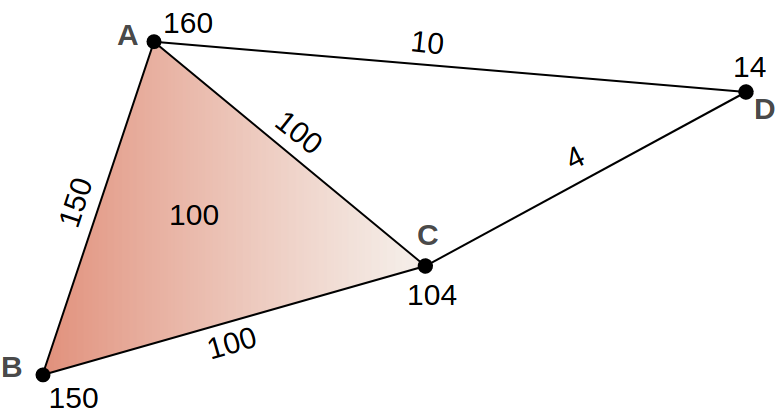
\includegraphics[height=2.3cm]{./figures/cc1.png}}%
\settowidth{\tempwidth}{\usebox{\tempbox}}%
\hfil\begin{minipage}[b]{\tempwidth}%
\raisebox{-\height}{\usebox{\tempbox}}%
\scriptsize{\captionof*{figure}{(b)}}%
\label{fig:co-authoship-complex}%
\end{minipage}%
\vspace{5pt}
%\end{table*}
\savebox{\tempbox}{\scriptsize{
\begin{blockarray}{cccccc}
\tiny{AB} & \tiny{AC} & \tiny{AD} & \tiny{BC} & \tiny{CD} \\
\begin{block}{(ccccc)c}
  3 & 0 & 1 & 0 & 0 & \tiny{AB} \\
  0 & 3 & 1 & 0 & -1 & \tiny{AC} \\
  1 & 1 & 2 & 0 & 1 & \tiny{AD} \\
  0 & 0 & 0 & 3 & -1 & \tiny{BC}\\
  0 & -1 & 1 & -1 & 2 & \tiny{CD}\\
\end{block}
\end{blockarray}}}%
\settowidth{\tempwidth}{\usebox{\tempbox}}%
\hfil\begin{minipage}[b]{\tempwidth}%
\raisebox{-\height}{\usebox{\tempbox}}%
\scriptsize{\captionof*{figure}{(c)}}%
\end{minipage}%
%\end{table*}
\caption{Example of co-authorship complex and its $1$-Laplacian. (a) Data. (b) Co-authorship complex with corresponding cochains build from the data. (c) $1$-Laplacian associated to the co-authorship complex. }\label{fig:data2complex}
\end{figure}

%\subsection{Simplicial Laplacians}
\textbf{Simplicial Laplacians.} We are in this paper concerned with finite abstract simplicial complexes, although our method is applicable to a much broader setting, such as for example finite CW-complexes. \gard{I kinda liked the point that emphasized that the simplicial complexes don't need an embedding, but maybe there isn't space for it?}
%In particular, it is not necessary for the simplicial complexes to come equipped with some embedding into Euclidean spaces, nor do we demand that they triangulate a Riemannian manifold.
To define a discrete version of the Laplacian for simplicial complexes, one simply takes the linear adjoint of the coboundary map with respect to the inner product, defining $\delta_i^\ast:C^{i+1}(K)\to C^i(K)$ by \gard{Do we need to tell people this? Can't we assume that the readers know linear algebra and just say that $\delta_i^\ast$ is the adjoint wrt.\ the IP, since we're short on space?}
\begin{equation*}
  \ip{\delta_i f_1}{f_2}_{i+1} =\ip{f_1}{\delta_i^\ast f_2}_{i},\ \forall f_1\in C^{i}(K), f_2 \in C^{i+1}(K).
\end{equation*}
\stefania{Kathryn: What about saying that the coboundary has a matrix representation and then just define the adjoint as its transpose? This involves the choice of a basis but it would make it easier to read for computer scientists.}

In analogy with Hodge--de Rham theory~\cite{madsen1997calculus}, we then define the \emph{degree-$i$ simplicial Laplacian} of a simplicial complex $K$ as the linear map $\lap_i:C^i(K)\to C^i(K)$ with
\begin{equation*}
  \lap_i = \lapu_i + \lapd_i = \delta_{i}^\ast\circ\delta_{i} + \delta_{i-1}\circ\delta_{i-1}^\ast.
\end{equation*}
\gard{I changed this formulation to save some space, feel free to revert.}
In the case $i=0$, $\mathcal{L}_0$ corresponds to the classical graph Laplacian. Observe that there are $p$ Laplacians for a complex of dimension $p$. \gard{Is the previous sentence really important?} \stefania{Kathryn: What about moving the following paragraph in the appendix?}In most practical applications, the matrices for the Laplacians are very sparse and can easily be computed as a product of sparse coboundary matrices and their transposes. Since the Laplacians encode information about the adjacency of the simplices, they can be interpreted as a message passing functions~\cite{gilmer2017NeuralMP}. Additionally, they carry valuable topological information about the simplicial complex. In particular, the kernel of the $k$-Laplacian is isomorphic to the $k$-(co)homology of its associated simplicial complex~\cite{eckmann1944,horak2013spectra}.
% In other words, the number of zero-eigenvalues tells us the number of $k$-dimensional holes~\cite{horak2013spectra}.


\paragraph{Simplicial convolution.}

A convolutional layer is of the form $\psi\circ(f\ast \varphi_W)$, where $\ast$ denotes convolution, $\varphi_W$ is a function
\emph{with small support} parameterized by learnable weights $W$, and $\psi$ is some nonlinearity and bias. This formulation of CNNs lends itself to a spectral interpretation that we exploit to extend CNNs to a much more general setting.

Following~\cite{defferrard2016convolutional} and motivated by the fact that the discrete Fourier transform of a real-valued function on an $n$-dimensional cubical grid coincides with its decomposition into a linear combination of the eigenfunctions of the graph Laplacian for that grid, we define the Fourier transform of real $p$-cochains on a simplicial complex with Laplacians $\mathcal{L}_p$ as
\begin{align*}
  &\mathcal{F}_p: C^p(K) \to \mathbb{R}^{\lvert K_p \rvert} \\
  &\mathcal{F}_p(c) = \left(\ip{c}{e_1}_p, \ip{c}{e_2}_p, \dotsc, \ip{c}{e_{\lvert K_p \rvert}}_p\right),
\end{align*}
where the $e_i$'s are the eigencochains of $\mathcal{L}_p$ ordered by eigenvalues $\lambda_1\leq\dotsm\leq\lambda_{\lvert K_p \rvert}$. The function $\mathcal{F}_p$ is invertible since $\mathcal{L}_p$ is diagonalizable; explicitly, if we write $U\diag(\Lambda)U\transpose$ for a normalized eigendecomposition, the orthonormal matrices $U$ and $U\transpose$ represent $\mathcal{F}\inv_p$ and $\mathcal{F}_p$, respectively. This is the foundation for Barbarossa's development of signal processing on simplicial complexes~\cite{barbarossa2018learning}.

Recall that on the function classes for which it is defined, the classical Fourier transform satisfies $\mathcal{F}(f\ast g)=\mathcal{F}(f)\mathcal{F}(g)$, where the right-hand side denotes pointwise multiplication. This will be our definition of convolution in the simplicial setting. Indeed, for cochains $c,c'\in C^p(K)$ we \emph{define} their convolution as the cochain
\begin{equation*}
  c\ast_p c' = \mathcal{F}_p\inv\left(\mathcal{F}_p(c)\mathcal{F}_p(c')\right). 
\end{equation*}

Within this framework, we are led to define a \emph{simplicial convolutional layer} with input $p$-cochain $c$ and weights $W$ as being of the form
\begin{equation*}
  \psi\circ\left(\mathcal{F}\inv_p(\varphi_W)\ast_p c\right)
  \end{equation*}
for some as of yet unspecified $\varphi_W\in\mathbb{R}^{\lvert K_p \rvert}$. To ensure the central property that a convolutional layer be localizing, we demand that $\varphi_W$ be a low-degree polynomial in $\Lambda=(\lambda_1, \dotsc, \lambda_{\lvert K_p \rvert})$, namely
\begin{equation*}
  \varphi_W = \sum_{i=0}^N W_i\Lambda^i = \sum_{i=0}^N W_i(\lambda^i_1, \lambda^i_2, \dotsc, \lambda^i_{\lvert K_p \rvert}),
\end{equation*}
for small $N$. In signal processing parlance, one would say that such a convolutional layer \emph{learns filters that are low-degree polynomials in the frequency domain}.

The reason for restricting the filters to be these low-degree polynomials is best appreciated when writing out the convolutional layer in a basis. Let $L^i_p$ denote the $i$'th power of the matrix for $\mathcal{L}_p$ in, say, the standard basis for $C^p(K)$, and similarly for $c$. Then (ignoring the nonlinearity $\psi$), 
\begin{equation*}
  \mathcal{F}\inv_p(\varphi_W)\ast_p c = \sum_{i=0}^N W_iU\diag(\Lambda^i)U\transpose c = \sum_{i=0}^N W_i\left(U\diag(\Lambda)U\transpose\right)^i c = \sum_{i=0}^NW_iL^i_pc. %\label{eq:filter}
\end{equation*}
This is important for three reasons, like for traditional CNNs.
First, the convolution can be efficiently implemented by $N$ sparse matrix-vector multiplications: This reduces the computational complexity from $\mathcal{O}(\lvert K_p\rvert^2)$ to $\mathcal{O}(\xi\lvert K_p\rvert)$ where $\xi$ is the density factor.
Second, the number of weights to be learned is reduced from $\mathcal{O}(\lvert K_p\rvert)$ to $\mathcal{O}(1)$.
Third, the operation is $N$-localizing in the sense that if two simplices $\sigma,\tau$ are more than $N$ hops apart, then a degree-$N$ convolutional layer does not cause interaction between $c(\sigma)$ and $c(\tau)$ in its output (see the supplementary material).
Those local interactions (in the spatial domain) can be interpreted as message-passing between simplices.%~\cite{gilmer2017NeuralMP}.

%In practice we implement \refeq{filter} using Chebyshev polynomials, as suggested for GNNs in~\cite{defferrard2016convolutional}.
%\mdeff{Not very important: The choice of polynomial (monomials, Chebyshev, Legendre, etc.) doesn't make much difference in practice.}

